\chapter{Parallel Plane Waveguide (2)}\label{lec:lec36}
We continue with our investigation of the propagation of electromagnetic waves inside a parallel plane waveguide. i.e. two conducting boundaries with waves moving in between them. In the previous chapter, we launched a wave which had perpendicular polarization between two conducting boundaries; as a result, we get a propagation which we call transverse electric propagation.

We introduced the concept of mode i.e. the discrete electric and magnetic field patterns which propagate between these two conducting boundaries. \emph{What if we use a parallel polarized electric field instead of perpendicular polarization? What kind of propagation will take place and how does it differ from the previous case of perpendicular polarization?} Figure~\ref{fig:silas1} shows a conductor boundary with the incident and reflected wave. The coordinate system is shown with y pointing out of the paper and as such the electric field is directed in the plane of the paper. Since this is a transverse wave, by Poynting theorem, the magnetic field for both must be in the y direction.
\begin{figure}[h]
\centering
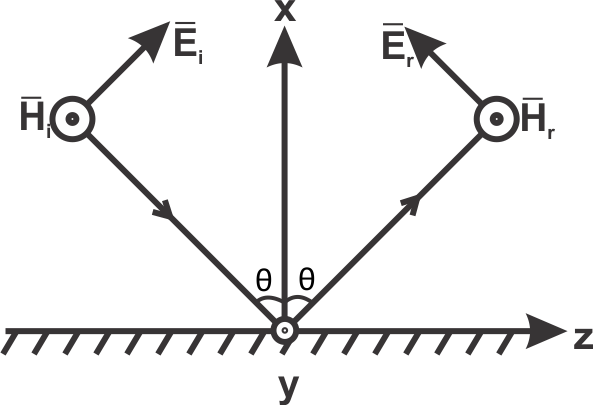
\includegraphics[scale=1]{\pathtoparttwo/graphics/silas1}
\caption{Incident and reflected wave on a boundary that lies in the z plane}
\label{fig:silas1}
\end{figure}

The problem is identical to what we had in the previous case. We find out the component of electric and magnetic fields and apply the boundary conditions.
\begin{figure}[h]
\centering
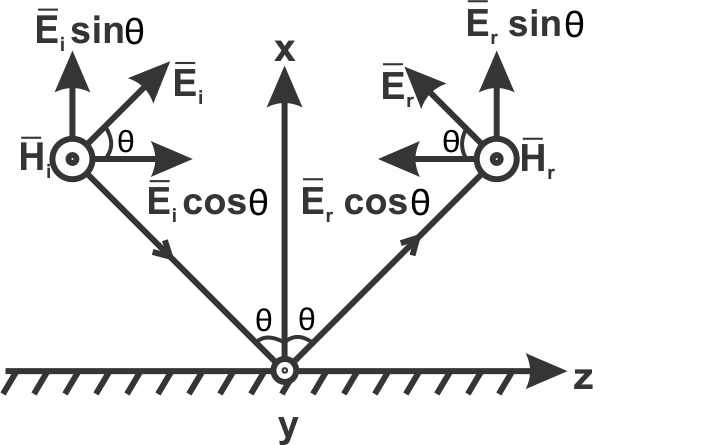
\includegraphics[scale=1]{\pathtoparttwo/graphics/silas2}
\caption{Incident and reflected wave with projected electric fields in the rectangular coordinate system}
\label{fig:silas2}
\end{figure}
At x = 0, the tangential component of the electric field should be zero.
\begin{equation*}
\bar{H_{i} = H_{i} e^{-j\beta(-xcos\theta + zsin\theta)} \hat{y}}
\end{equation*}
\begin{equation*}
\bar{H_{r} = H_{r} e^{-j\beta(-xcos\theta + zsin\theta)} \hat{y}}
\end{equation*}
\begin{equation*}
\bar{E_{i} = E_{i} e^{-j\beta(-xcos\theta + zsin\theta)} \hat{y}}
\end{equation*}
\begin{equation*}
\bar{E_{r} = E_{r} e^{-j\beta(-xcos\theta + zsin\theta)} \hat{y}}
\end{equation*}
Taking the component of the incident electric field in the z direction, we have $E_{i} cos\theta$ and $-E_{r}cos\theta$ for the reflected electric field in the z-direction also.\\
$E_{iz} = E_{i}cos\theta e^{-j\beta(-xcos\theta + zsin\theta)}$	for the boundary condition and x = 0\\
$E_{rz} = -E_{r}cos\theta e^{-j\beta(xcos\theta + zsin\theta)}$   Sum of tangential electric field is zero.\\
At x = 0, $E_{ton} = E_{iz} + E_{rz}$\\
If we substitute, we have\\
\begin{equation*}
E_{i}cos\theta e^{-j\beta(-xcos\theta + zsin\theta)} - E_{r}cos\theta e^{-j\beta(xcos\theta + zsin\theta)} = 0
\end{equation*}
as x$\rightarrow$
\begin{equation*}
E_{i}cos\theta e^{-j\beta(zsin\theta)} - E_{r}cos\theta e^{-j\beta(zsin\theta)} = 0
\end{equation*}
\begin{align*}
E_{i} = E_{r}\\
\Gamma= 1 = \frac{E_{i}}{E_{r}}
\end{align*}
We recall that we have a reflection coefficient $\Gamma = -1$ in the case of perpendicular polarization. This means it was behaving like a short circuit. For the parallel polarization, the transmission line analogy is an open circuit? which is not correct. The $E_{i}$ and $E_{r}$ from the diagram have a direction opposite to each other. So that in the case of perpendicular polarization, the $E_{i}$ and $ E_{r}$  were initially taken to be in the positive y direction. So   $\Gamma = 1$ means they are opposite to one another in direction, so n = -1 corresponded to the case of a short circuit in Transmission lines. Hence the negative sign that could have been in $\Gamma$ here is already taken care of by making $E_{i}$ and $E_{i}$ have opposite directions in the case of parallel polarization considered here. Thus, the reason the reflection coefficient is 1. 

Looking at the sign of the reflection coefficient alone will not give the correct idea about the boundary. In summary, this parallel polarized case is still behaving like a short circuit, where the conductivity is infinite. The electric field is zero at the boundary, you get a reflection coefficient of +1 because the sign is appropriately absorbed into the direction of the electric field. Once you get that and use the relationship that the electric field is related to the magnetic field by the intense importance, we have $\frac{E_{i}}{H_{i}} = \frac{E_{r}}{H_{r}} =\Gamma$. The total electric field in medium 1 is a summation of the incident and reflected field. The same is true for the magnetic field. The electric field has two components in x and z, and the magnetic field has components in only y duration. The magnetic field will have only the y component.
\begin{equation*}
E_{i}sin\theta e^{-j\beta(-xcos\theta + zsin\theta)} + E_{r}sin\theta e^{-j\beta(xcos\theta + zsin\theta)}
\end{equation*}
$E_{i} =E_{r}$    since $\Gamma =1$\\
we have
\begin{dmath*}
E_{r}sin\theta [e^{-j\beta(-xcos\theta} + e^{-j\beta cos\theta}] e^{-j\beta(zsin\theta)} = 2E_{i}sin\theta cos(\beta xcos\theta)
\end{dmath*}
therefore,
\begin{dmath*}
E_x = 2E_{i}sin\theta cos(\beta xcos\theta)
E_{2} is E_{i}cos\theta e^{-j\beta(-xcos\theta + zsin\theta)} - E_{r}cos\theta e^{-j\beta(xcos\theta + zsin\theta)} 
\end{dmath*}
\begin{dmath*}
= E_{i}cos[e^{j\beta xcos\theta} - e^{-j\beta xcos\theta}]e^{-j\beta zsin\theta}
=2jE_{i}e^{-j\beta zsin\theta} cos\theta \times sin(\beta xcos\theta)
\end{dmath*}
The magnitude field will have only y component
\begin{equation*}
H_{y} = H_{i}e^{-j\beta(-xcos\theta + zsin\theta)} + H_{r}e^{-j\beta(+xcos\theta + zsin\theta)}
\end{equation*}
since $\Gamma = 1 that is E_{i}=E_{r}$
\begin{equation*}
= \frac{E_{i}}{\eta} e^{-j\beta(-xcos\theta + zsin\theta)} + \frac{E_{i}}{\eta}e^{-j\beta(+xcos\theta + zsin\theta)}
\end{equation*}
\begin{equation*}
=\frac{E_{i}}{\eta} e^{-j\beta(-zsin\theta)} [e^{j\beta xcos\theta} + e^{-j\beta xcos\theta}]
\end{equation*}
\begin{equation*}
= 2\frac{E_{i}}{\eta} cos(\beta xcos\theta)e^{-j\beta zsin\theta}
\end{equation*}
So we have the three equations
\begin{equation}
E_x = 2 E_{i} e^{-j\beta zsin\theta} sin\theta cos(\beta xcos\theta)
\label{eqn:field1}
\end{equation}
\begin{equation}
E_z = 2 jE_{i} e^{-j\beta zsin\theta} sin\theta cos(\beta xcos\theta)
\label{eqn:field2}
\end{equation}
\begin{equation}
H_y = 2 \frac{E_{i}}{\eta} cos(\beta xcos\theta) e^{-j\beta zsin\theta} 
\label{eqn:field3}
\end{equation}
If we look at the tangential component of the electric field $E_{2}$, this is going to be zero at x = 0. That is when $sin(\beta xcos\theta) =0$ or $\beta xcos\theta = m\pi$ where m = 0,1,2.... The angle at which the parallel polarization can be launched to propagate the wave becomes discrete angles given as $cos\theta = \frac{m\pi}{\beta x}$. If the separation between the conducting plane 'x' is given, i.e. x = d, then we can launch the wave at discrete angle =0 for m=0,1,2,3... Whether we take a parallel polarization, the angles at which the wave can be launched inside the structure remain the same for either case. All the arguments we have in the previous case like you have a finite number of angles in which the wave can be launched, and the minimum value of frequency required, all those arguments are applicable here too. With waveguide separation $d$, $cos\theta$ = $\frac{m\pi}{\beta d}$.
%\begin{figure}[h]
%\centering
%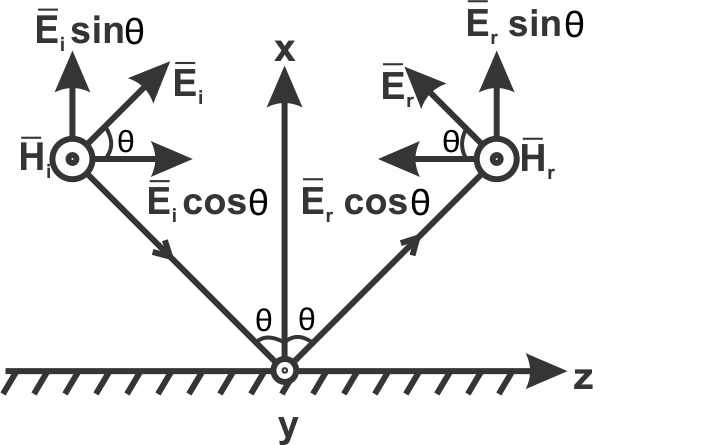
\includegraphics[scale=1]{\pathtoparttwo/graphics/silas2}
%\caption{}
%\end{figure}
From figure~\ref{fig:silas2}, the magnetic field component is always perpendicular to the plane of incidence, while the electric field i.e. on the plane of the paper. $cos(\beta xcos\theta)$ represents an expression for a standing wave in the x-direction and $e^{-j\beta zsin\theta}$ gives a travelling wave behaviour in the z-direction. So in this case our field will travel in the z-direction, with a phase constant $\beta sin\theta$. So a field parallel is generated also if a conducting wave is placed at distance $d= \frac{m\lambda}{z cos\theta}$, that is travelling with a phase constant $\beta sin\theta$ in the z-direction. Since the wave is travelling in the z-direction and the magnetic field is now perpendicular to the direction of travel along all points within these two conducting boundaries, the magnetic field is always transverse to the direction of no propagation of the electromagnetic wave. This mode is called a \textbf{Transverse Magnetic} mode or TM mode.

\section{Tranverse Magnetic  Modes ($TM_m$)}\index{Transverse Magnetic Modes}
 Following the convention, $m$ defines the order of the mode i.e. tells us how many no of half cycles variation we have from $x = 0$ to $x = d$.
\begin{figure}[h]
\centering
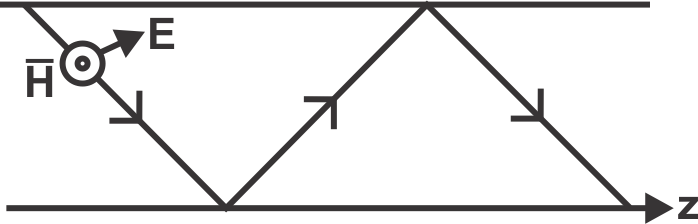
\includegraphics[scale=1]{\pathtoparttwo/graphics/silas3}
\caption{Transverse magnetic  mode}
\end{figure}
Hence, $ m = 1$ means 1 half-cycle variation between $x = 0$ and $x = d$, $m = 2$ means 2 half-cycle variations between $x = 0$ and $x = d$, and when $m = 0$, the fields are constant with no variation. This is represented as $TM_m$. 

For a given value of $d$, the value of $m$ we choose to execute the fields will decide the order of the mode of propagation. Now we see that we have two types of propagation inside a parallel plane waveguide. The transverse electric mode $TE$ and the transverse magnetic mode $TM$ for which electric and magnetic field remains transverse to the direction of net wave propagation respectively. 

Up till now, the behaviour is very identical. They have the same condition satisfied for the electric field, but the magnetic and electric field expressions are different. Otherwise no difference between $TE$ or $TM$ modes. With $x = d$,
\begin{dmath*}
cos\theta = \frac{m \pi}{\beta d} =\frac{m \pi}{\frac{2\pi d}{\lambda}} = \frac{m\lambda}{2d}
\end{dmath*} 
or
\begin{dmath*}
\beta cos\theta = \frac{m \pi}{d}
\end{dmath*}
We substitute for $\beta cos\theta$ in the field equations \ref{eqn:field1}, \ref{eqn:field2}, and \ref{eqn:field3}.
\begin{dmath}
E_{x} = 2 E_{i} e^{-j\beta zsin\theta} sin\theta cos(\beta xcos\theta) = 2 E_{i} e^{-j\beta zsin\theta} sin\theta cos(\frac{m\pi x}{d})
\end{dmath}
\begin{dmath}
E_{2} = 2 jE_{i} e^{-j\beta zsin\theta} sin\theta cos(\beta xcos\theta) = 2 jE_{i} e^{-j\beta zsin\theta} sin\theta cos(\frac{m\pi x}{d})
\end{dmath}
\begin{dmath}
H_{y} = 2 \frac{E_{i}}{\eta} cos(\beta xcos\theta) e^{-j\beta zsin\theta} =2 \frac{E_{i}}{\eta} cos(\frac{m\pi x}{d}) e^{-j\beta zsin\theta} 
\end{dmath}
Again, $m$ gives the number of half-cycle variations between $x = 0$ and $x = d$. In the transverse electric case with $m = 0$, ALL THE FIELDS BECAME ZERO. Thus, the $TE_0$ mode cannot exist inside a parallel plane waveguide. In this case if we put $m = 0$, then $cos\theta =0$, $\theta =90$, that means $sin\theta =1$. The wave will move parallel to the conducting boundary. In this case of $m = 0$, $cos\theta =0$ and $sin\theta =1$ and $\theta=\frac{\pi}{2}$ , so we have for $TM_0$\\ 
$E_{x} =2E_{i} e^{-j\beta z}$, $E_{z}= 0$, $H_{y} =\frac{2E_{i}}{\eta} e^{-j\beta z}$.

Here the phase constant is the same as we have for the intrinsic medium filling the parallel plane waveguide. We notice that when $m = 0$, all the fields do not identically go to zero. That means $TM_0$ mode does exist so contrary to $TE_0$ mode which does not exist, and subsequently, we have $TM_{1}$, $TM_{2}$, and so on. 

\section{Phase and Group Velocities}\index{Phase and Group Velocities}
Phase constant in the z-direction is
\begin{dmath*}
\bar{\beta} = \beta\sin\theta = \beta \sqrt{1- cos^{2}\theta} =\beta\sqrt{1 - \left(\frac{m\lambda}{2d}\right)^{2}}
\end{dmath*}
This is the phase constant for the transverse magnetic case, with $m = 0$, $\bar{\beta}$ reduces to $\beta$ here. With $m\neq 0$, we can ask with what velocity this particular mode will be travelling. Thus, we define velocity by group velocity $v_{g}$ or by phase velocity $v_{p}$. 
\begin{dmath}
 v_{p}=\frac{\omega}{\bar{\beta}} =\frac{\omega}{\beta \sqrt{1 - \left(\frac{m\lambda}{2d}\right)^{2}}}
\label{eqn:phasevel}
\end{dmath}
$\beta$ is the phase constant in the medium filling the two conducting planes, $\frac{\omega}{\beta}$ is the velocity of a wave in an unbound medium having the same property, and $\frac{\omega}{\beta}$ is the velocity of light, $c$. Thus equation~\ref{eqn:phasevel} becomes;
\begin{equation*}
v_{p} =\frac{c}{\beta\sqrt{1 - \left(\frac{m\lambda}{2d}\right)^{2}}}
\end{equation*}
But 
\begin{align}
v_{p} v_{g}= c^{2}
\label{eqn:grpvel}
\end{align}
$v_{g}$ is the group velocity. In the parallel plane waveguide shown in figure~\ref{fig:silas4}, with the wave going at an angle $\theta$, the component of the wave in the z-direction gives the group velocity of the wave in the z-direction in the parallel plane waveguide. The velocity of the wave in the $\theta$ direction is $c$. So that $c\times \cos(\frac{\pi}{2} - \theta)= c\times \sin\theta= v_{gz}$. The group velocity is the component of the velocity in the z-direction.
\begin{figure}[h]
\centering
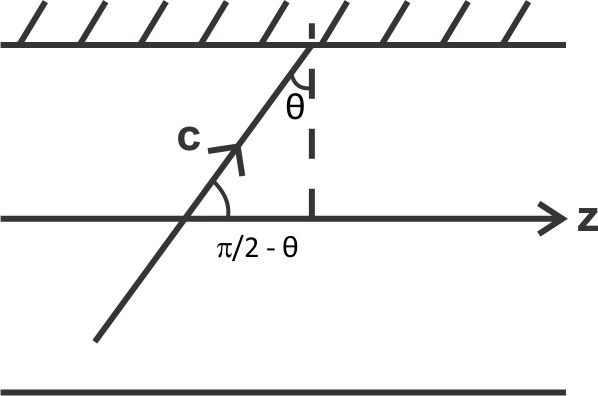
\includegraphics[scale=1]{\pathtoparttwo/graphics/silas4}
\caption{Group velocity of a wave propagating in a medium bounded by a parallel plane in the z plane}
\label{fig:silas4}
\end{figure}
From equation~\ref{eqn:grpvel}, we can derive the group velocity as:
\begin{dmath}
v_g = \frac{c^2}{v_p} = \frac{c^2}{\frac{c}{\sin\theta}}= c\sqrt{1-\cos^{2}\theta} =c\sqrt{1-\left(\frac{m\lambda}{2d}\right)^{2}}
\label{eqn:grpvel2}
\end{dmath}
The group velocity is the velocity of the energy. We note two things from these expressions, if $m \neq 0$, the phase velocity is a function of wavelength. For a given mode,$m \neq 0$ when the frequency changes, the phase velocity of that particular mode changes. The property of velocity of a wave changing as a function of frequency is called \textbf{Dispersion}\index{Dispersion}. 

\subsection{Dispersion}
What we find is when we have a medium like this parallel plane waveguide, the structure has become a dispersive structure. This is when electromagnetic wave tires move in the structure, the velocity becomes a function of frequency or function of wavelength. So though the medium feeling this waveguide is not dispersive, the conducting boundary or dial conductors we talked about are not also dispersive, but this bound medium has become a dispersive medium. When we have a bounded structure, in general, we may expect dispersion on the bound structure i.e. their velocity varies as a function of frequency. Hence, neither the medium within the conductor nor the conducting plane itself is dispersive, but the \textbf{Bounded Structure} formed with all these have become \textbf{Dispersive}.
\begin{equation}
\bar{\beta} = \sqrt{\beta^{2} -\left(\frac{m\pi}{d}\right)^{2}}
\end{equation} 
This is called the \textbf{Dispersion Relation} for a particular mode, it tells the variation of velocity as a function of frequency or wavelength. The conclusion is that whenever we have a bound structure, the velocity varies as a function of frequency or wavelength.

$(\frac{m\lambda}{2d})^{2} -1=0$ gives the cut-off wavelength, and at $\beta^{2} -(\frac{m\pi}{d})^{2}$, the wave propagation will stop. For a frequency lower, wave propagation does not take place and for a higher frequency than $f_{cut-off}$, the wave propagates. As we approach cut-off frequency, $v_{p}\Rightarrow \infty$ i.e $v_{p}= \frac{c}{\beta \sqrt{1- \left(\frac{m \lambda}{2d}\right)^{2}}}$ at cut-off $1 - (\frac{m\lambda}{2d})^{2}=0$ $v_{p} =\frac{c}{0} =\infty$

$v_{g} =c \sqrt{1-(\frac{m\lambda}{2d})^{2}}$ $\Rightarrow 0$. With $v_{g} = 0$ it means at cut-off, the energy flow stops. At frequencies very high compared to cut-off frequencies, $\lambda$ becomes very very small compared to cut-off, $\frac{m\lambda}{2d} \rightarrow 0$ becomes negligibly small,$v_{g} \approx c$, $v_{p} \approx c$. so at higher frequencies compared to cut-off frequency, $v_{g}$ and $v_{p}$ approaches the intrinsic velocity in the medium.
\begin{figure}[h]
\centering
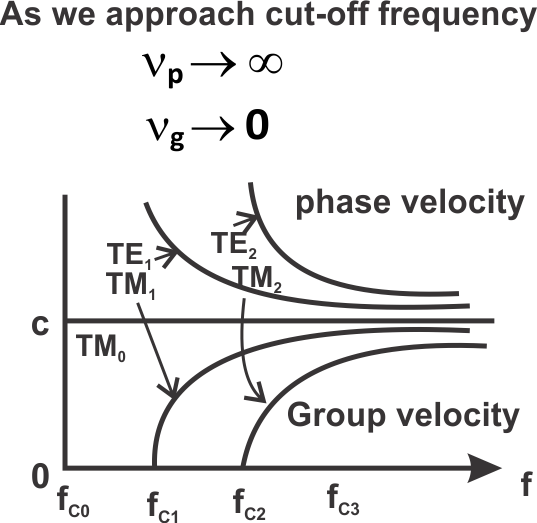
\includegraphics[scale=1]{\pathtoparttwo/graphics/silas5}
\caption{Group and phase velocities versus frequency at different $TE$ and $TM$ modes}
\label{fig:silas5}
\end{figure}
A plot of group and phase velocity for different frequencies is shown in figure~\ref{fig:silas5}. $f_{c1}$ is the cut-off frequency for mode $m=1$, $f_{c2}$ is the cut-off frequency for mode $m=2$, $f_{c0}$ is the cut-off frequency for mode $m=0$ which exists for only $TM$ since $TE_0$ does not exist.

From equation~\ref{eqn:phasevel}, we can see that if $m=0$, $v_{p} =c$ ($TM_0$ since $TE_0$ does not exist). For $m=1$
\begin{equation*}
v_{p}= \frac{c}{\beta \sqrt{1- \left(\frac{\lambda}{2d}\right)^{2}}}
\end{equation*}
As $v_{p}$ approaches $c$, starting from $\infty$ at $f_{c1}$, $v_{g}$ approaches $c$ starting from 0 at $f_{c1}$.
\begin{equation*}
v_{g}= c\sqrt{1-\left(\frac{\lambda}{2d}\right)^{2}}
\end{equation*}
At cut-off frequency, 
\begin{align*}
1-\left(\frac{m\lambda}{2d}\right)^{2} = 0
\end{align*}
Therefore, at every cut-off for the respective mode, $v_{p}$ starts from $\infty$ and tends to $c$ as $f$ increases, $v_{g}$ starts from 0 and approaches $c$ as f increases. $TM_{1}$, and $TE_{1}$, do exist, But $TE_0$ does not exist when $TM_0$ exists. For $m = 0$, $v_{p}=c$ $v_{g}=c$. The phase velocity is always above $c$ and the group velocity is always below $c$.

The graph in figure~\ref{fig:silas5} shows the group and phase velocity plot for the different modes, where $f_{c0}$, $f_{c1}$, and $f_{c2}$ are the cut-off frequencies for the different modes. For the $TM_0$ mode, there is no cut-off frequency because $\bar{\beta}$ is always equal to $\beta$ which is the phase constant in the intrinsic medium. With this understanding, we go back to all the special cases we have talked about. Recall with $m = 0$, 
\begin{align*}
E_{x} =2E_{i} e^{-j\beta z}\\
H_{y} = \frac{2E_{i}}{\eta} e^{-j\beta z}\\
H_{z} =0
\end{align*}
This is the $TM_0$ mode. For the $TM_0$ mode, we draw the parallel plane waveguide to illustrate it $\theta =90^{0}$ means the wave is launched parallel to the interface as shown in figure~\ref{fig:silas6}

\begin{exmp}
\subsubsection*{Modes in a parallel-plate waveguide}
Consider a dielectric-filled parallel-plate waveguide with d = 2cm. The permeability of the dielectric filling is $\mu_0$ and its refractive index is n = 1.5.
\begin{enumerate}[(a)]
\item Which TE$_m$ and TM$_m$ modes can propagate a 12 GHz signal in the waveguide?
\item What would be the associated cutoff wavelengths in each case?
\item What would be the associated group velocities in each case?\textemdash here assume a modulated 12 GHz carrier with a narrow modulated bandwidth.
\end{enumerate}

\subsubsection*{Solution}
\begin{dmath*}
\text{Cutoff frequencies for modes, m, }f_{c_m} = \frac{mc}{2d}\quad\text{(for air-filled dielectric)}
\end{dmath*}
For the dielectric medium of refractive index, the cutoff frequencies for mode, m is given by
\begin{dmath*}
f_{c_m} = \frac{m\left(\dfrac{c}{n}\right)}{2d} = \frac{m\left(\dfrac{3 \times 10^8}{1.5}\right)}{2\times 0.02} = \frac{10^{10}}{2}m = 5m GHz
\end{dmath*}
So the modes that will propagate are cutoff frequencies less than 12 GHz at m values.

At m = 1
\begin{dmath*}
f_{c_1} = 5 GHz\quad\text{(will propagate)}
\end{dmath*}
At m = 2
\begin{dmath*}
f_{c_2} = 5\times2 = 10 GHz\quad\text{(will propagate)}
\end{dmath*}
At m = 3
\begin{dmath*}
f_{c_1} = 5\times3 = 15 GHz\quad\text{(will not propagate)}
\end{dmath*}
Hence, only 2 modes (TE/TM)$_{1,2}$ will propagate besides TEM mode which is true for all frequencies.

\paragraph{(b)} The associated wavelengths for both modes are
\begin{dmath*}
\lambda_{c_m} = \frac{v}{f_{c_m}} = \frac{2d}{m}
\end{dmath*}
At m = 1
\begin{dmath*}
\lambda_{c_1} = 2\times0.02=0.04 m
\end{dmath*}
At m = 2
\begin{dmath*}
\lambda_{c_2} = 2\times\frac{0.02}{2} = 0.02 m
\end{dmath*}

\paragraph{(c)} The group velocity is given as
\begin{align*}
v_g = c\sqrt{1 - \left(\frac{m\lambda}{2d}\right)^2}\quad\text{(for air-filled dielectric)}
\end{align*}
For the dielectric medium of refractive index, n, the group velocity is
\begin{align*}
v_g = \frac{c}{n}\sqrt{1 - \left(\frac{m\lambda}{2d}\right)^2}
\end{align*}
Recall $f_c = \frac{m\left(\frac{c}{n}\right)}{2d}$
\begin{dmath*}
v_g = \sqrt{\left(\frac{c}{n}\right)^2 - \left(\frac{m\lambda\frac{c}{n}}{2d}\right)^2}
= \sqrt{\left(\frac{c}{n}\right)^2 - (\lambda f_{c_m})^2}\quad\text{But $\lambda = \frac{\frac{c}{n}}{f}$}
\end{dmath*}
\begin{dmath}
\text{So, }v_g = \frac{c}{n}\sqrt{1 - \left(\frac{f_{c_m}}{f}\right)^2}
\label{eqn:grpvel3}
\end{dmath}
For $f_c = 5$ GHz at m = 1,
\begin{dmath*}
v_g = 2\times10^8\sqrt{1 - \left(\frac{5}{12}\right)^2} = 1.82\times10^8 m/s
\end{dmath*}
For $f_{c} = 10$ GHz at m = 2,
\begin{dmath*}
v_g = 2\times10^8\sqrt{1 - \left(\frac{10}{12}\right)^2} = 1.11\times10^8 m/s
\end{dmath*}
At m = 0, special case TEM mode,$v_g = v = 2\times10^8$ m/s.
\end{exmp}

\section{Transverse Electromagnetic Mode $TEM$}\index{Transverse Electromagnetic Mode}
\begin{figure}[h]
\centering
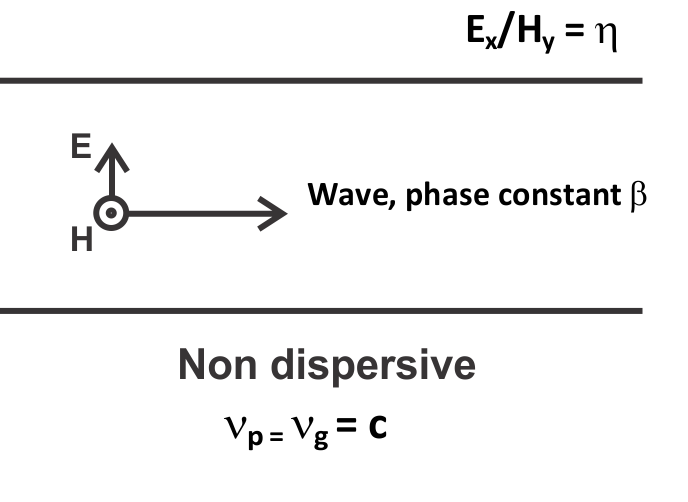
\includegraphics[width=1\linewidth]{\pathtoparttwo/graphics/silas6}
\caption{Wave propagation in $TM_0$}
\label{fig:silas6}
\end{figure}
The electric field is x-oriented, and the magnetic field is y-oriented i.e. pointing out of the plane of the paper. The wave is propagating in the z-direction with a phase constant $\beta$. We note that $\frac{E_{x}}{H_{y}} = \eta$. We see that in this case, the electric and magnetic field is now perpendicular to the direction of wave propagation z, $E_{x}\perp z$,$H_{y}\perp z$, and $E_{x}\perp H_{y}$. Hence the $TM_0$ mode is a case of \textbf{Transverse Electromagnetic Wave} and so we can call it a $TEM$ mode (Transverse Electromagnetic mode). $TM_0$ mode from here makes the electric and magnetic field becomes transverse to the direction of propagation hence the reason it is called Transverse Electromagnetic mode (TEM). With $\frac{E_{x}}{H_{y}} = \eta$ it means we are having a transverse electromagnetic wave posing in between the two planes. It has all the properties a uniform plane wave has in an unbound medium.

A question that comes to mind is if the conducting boundary still has any effect on the wave propagation, since if the boundaries are not there the wave would have travelled like a transverse electromagnetic wave. When the wave is launched the way it is shown in figure~\ref{fig:silas6} with the electric field perpendicular to the boundary, there is no boundary condition on normal components of the electric field. The normal component of the electric field always tends to be balanced by surface charges on the conducting boundary. Similarly, if we have a tangential component of the magnetic field we can have surface circuits on the conducting boundary. This balances out the tangential magnetic field in the conducting boundary. Now we can have a uniform magnetic and electric field, the wave passes through the parallel plane waveguide as if the boundaries are not modifying the electric and magnetic fields. whichever electric and magnetic field we have, they can induce appropriate surface changes and current, and this field does not get modified. Hence this $TM_0$ mode propagates in a parallel plane waveguide, and since $m = 0$, this mode is \textbf{Non-dispersive}. That means for this mode, the velocity $v_{p}=v_{g}=c$. The cut-off frequency for this mode is zero as we have seen when m = 0. That means this mode can propagate down to zero frequency. Precisely, this is what we see when we are having a two-conductor plane system, any lowest possible frequency voltage can be applied to the system and the energy would still be transferred or transported. However, higher-order modes require a minimum frequency for transporting the energy. So we find that in a parallel plane waveguide, this $TM_0$ mode also called a TEM mode is a mode that propagates at the lowest frequency. As we go to higher frequencies, we require higher other modes or we get higher order modes in the energy propagation.

\section*{Exercises}
\begin{ExerciseList}
\Exercise[label={ex361}]
Using the field equations of a TM mode propagation in a parallel plane waveguide assuming an air-filled dielectric given by:
\begin{align*}
E_x &= 2E_ie^{-\beta z\sin\theta}\sin\theta\cos(\beta x\sin\theta)\hat{x}\\
E_z &= j2E_ie^{-\beta z\sin\theta}\cos\theta\sin(\beta x\sin\theta)\hat{z}\\
H_y &= \frac{2E_i}{\eta}e^{-\beta z\sin\theta}\cos(\beta x\sin\theta)\hat{y}
\end{align*}
Show that:
\begin{enumerate}[(a)]
\item TM$_0$ mode is a TEM mode
\item The cutoff frequency and cutoff wavelength of the TM$_0$ mode are zero and infinity respectively.
\item The phase velocity and group velocity of the TM$_0$ mode are equal to the speed of light.
\item The TM$_0$ mode is non-dispersive.
\end{enumerate}

\Exercise[label={ex362}]
Consider an air-filled parallel-plate waveguide with d = 3 cm. Calculate the guide wavelength, $\lambda_g$ or the attenuation rate in dB/cm of the TE$_1$ mode in the guide\textemdash whichever appropriate\textemdash if the operating wavelength of the mode is
\begin{enumerate}[(a)]
\item $\lambda = 3$ cm
\item $\lambda = 12$ cm
\end{enumerate}
(Take attenuation rate as $20\log_{10} e^{\bar{\beta}z}$)

\Answer[ref={ex362}]
(a) $\lambda_g = 2\sqrt{3}$ cm (b) attenuation rate = 7.88 dB/cm

\Exercise[label={ex363}]
A parallel-plate waveguide with d = 3 cm is air-filled for $z < 0$ but it is filled with a dielectric for $z > 0$ which has $\mu = \mu_0$ and a refractive index n = 1.5. If a TE$_1$ mode wave field with $\lambda = 3$ cm is incident from the air filled region on the interface at z = 0, what fraction of the time-average incident power will be transmitted into the $z > 0$ region of the waveguide.

\Answer[ref={ex363}]
0.942
\end{ExerciseList}
